\documentclass[11pt,a4paper,oneside]{article}


\usepackage[T2A]{fontenc}
\usepackage[utf8]{inputenc}
\usepackage[english,russian]{babel}
\usepackage[russian]{olymp}
\usepackage{graphics}
\usepackage{wrapfig}
\usepackage{amsmath}
\usepackage{amssymb}
\usepackage{epigraph}
\usepackage{graphicx}
\usepackage{multicol}


\newcommand{\qo}{\textquotesingle}
\newcommand{\qq}{\textquotesingle~}

\contest{ACM ICPC Kyrgyzstan Subregional 2015}{Бишкек}{1 ноября 2015 года}    

\binoppenalty=10000
\relpenalty=10000
\exhyphenpenalty=10000

\renewcommand{\t}{\texttt}

\createsection{\Note}{Примечание}

\renewcommand{\defaultmemorylimit}{256 мегабайт}

\begin{document}

\begin{problem}{Задача H. Площадь}{1 секунда}{32 мегабайта}

По данным натуральным числам  $P, Q \leq 100$ найти площадь области на плоскости, определенной 5-ю неравенствами:  $0 \leq X$; ~~ $0\leq Y$; ~~ $X+Y\leq 15$;~~ $X\leq P$;
~~ $Y \leq Q$;
и округлить ее до целого числа с избытком. 


\InputFile

Одна строка, в которой записаны два натуральных числа, разделенные одинарным пробелом.

\OutputFile
Одно натуральное число.


\Examples

\begin{example}%
\exmp{
10 6
}{
60
}%
\exmp{
20 10
}{
100
}%
\end{example}

\vspace{0.1cm}
\medskip\noindent
\textbf{Пояснение к примерам.}


Области, определенные неравенствами в первом и втором примерах, изображены на рисунках 1 и 2 соответственно.

\begin{figure}[ht]
\centering
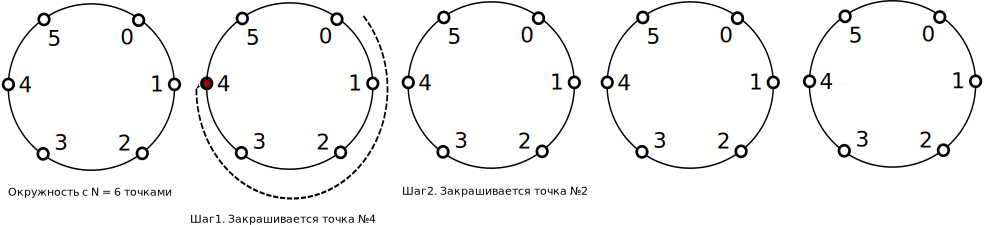
\includegraphics[width=0.4\textwidth]{drawing.pdf}
\caption{Область в первом
 примере}
\end{figure}

\vspace{-0.2cm}
\begin{figure}[ht]
\centering
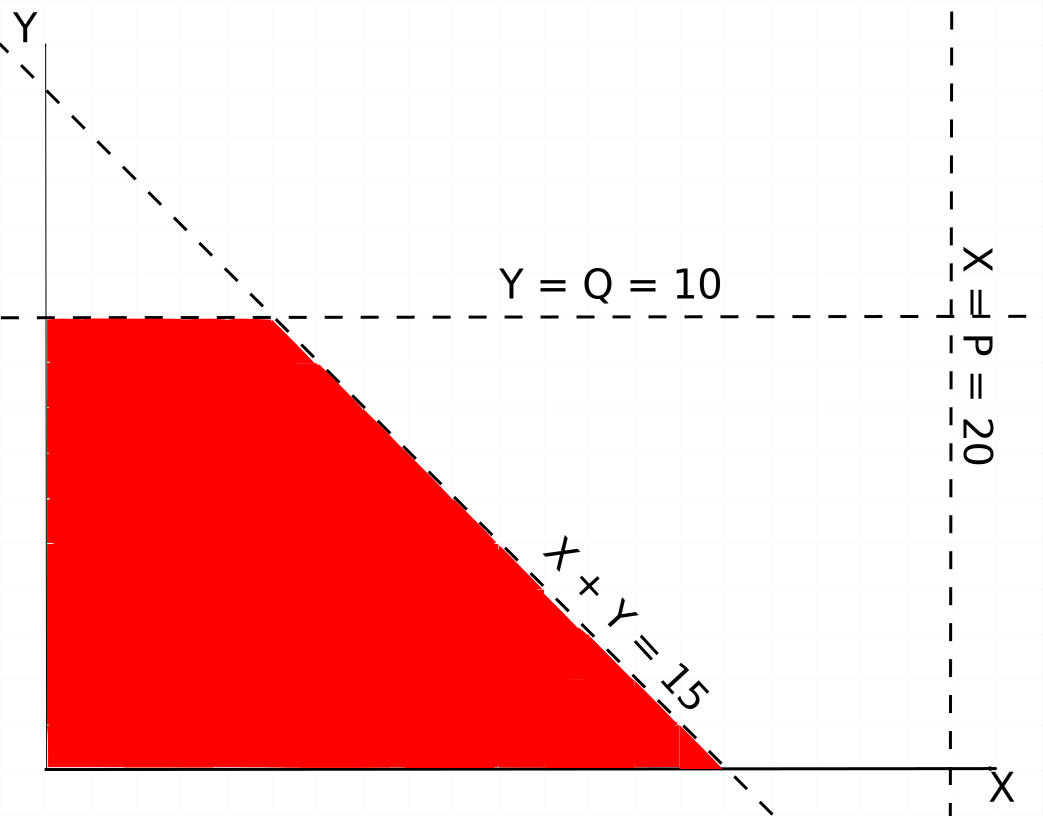
\includegraphics[width=0.4\textwidth]{drawing2.pdf}
\caption{Область во втором примере}
\end{figure}






\vspace{1.0cm}
\hfill \textit{Автор задачи: Панков П.C.}
\medskip\noindent




\end{problem}


\end{document}
%%% Local Variables:
%%% mode: latex
%%% TeX-master: t
%%% End:
